%  figure placement: here, top, bottom, or page
\begin{figure}
   \centering
   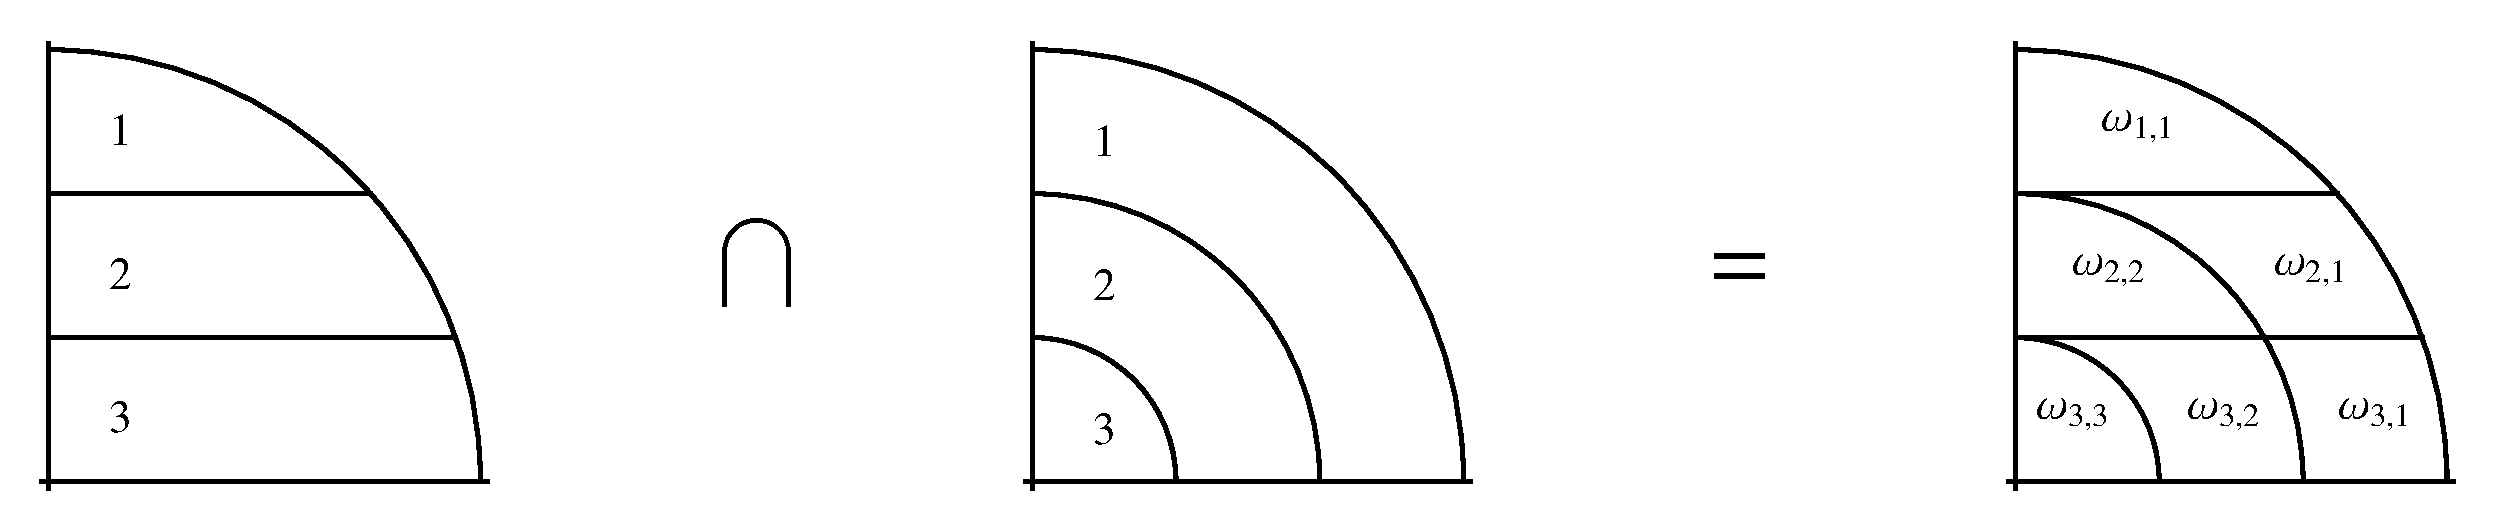
\includegraphics[ width = 5in ]{graphics/row.eps}  \\ \
   \emph{limbs, $\Lambda$} \qquad \qquad \qquad \qquad \qquad
   \emph{shells, $\Sigma$} \qquad \qquad \qquad \qquad \qquad
   \emph{sectors, $\omega_{\Lambda,\Sigma}$} \\[10pt]
   \caption{Sectors are created by the intersection of the horizontal partition (limbs) and the radial partition (shells). The numbering of the sectors $\omega_{\Lambda,\Sigma}$ is indexed to the location (limb, shell) in the capsule.}
   \label{fig:partition intersection}
\end{figure}

\endinput  %  .  .  .  .  .  .  .  .  .  .  .  .  .  .  .  .  .  .